\documentclass[10pt,a4paper,oneside]{article}

\usepackage{charter}
\usepackage{eulervm}
\usepackage{amsmath, amsthm, amssymb}
\usepackage{graphicx}
\usepackage{caption}
\usepackage{subcaption}

\theoremstyle{definition}
\newtheorem*{thm}{Theorem}
\newtheorem{lma}{Lemma}
\newtheorem*{dfn}{Definition}
\newtheorem*{exm}{Example}

\usepackage{color}
\usepackage[usenames,dvipsnames,svgnames,table]{xcolor}

\DeclareMathOperator*{\argmin}{arg\,min}
\DeclareMathOperator*{\argmax}{argmax}

\title{EM-algorithms for learning Discrete and Random Iterated Function Systems}
\date{\today}

% non-indented, spaced paragraphs
\setlength{\parindent}{0.0in}
\setlength{\parskip}{0.1in}

\begin{document}

\maketitle

\begin{abstract}
\noindent We present an algorithm for solving the \emph{inverse problem}, the task of finding a fractal model for a given data set. The algorithm is inspired by the famous Expectation Maximization algorithm for fitting models with hidden variables. We build on a connection between Mixture-of-Gaussian models and Iterated function Systems (IFSs) to design an EM-style algorithm for IFS models. We also extend our algorithm to fit Random Iterated Function Systems (RIFSs) to data.
\end{abstract}

\section*{Definitions}

We will briefly review the established definitions and basic properties of Iterated Function Systems and their random variant. As the properties are well established, we will forego their proofs. For a more extensive introduction, including proofs and detailed references, we recommend \cite{hutchinson2000deterministic}. 

\begin{dfn}{Iterated Function System (Set)}
An iterated function system $S$ is a set of $k$ contractive functions $S_i:{\mathbb R}^d \rightarrow {\mathbb R}^d$. The individual functions $S_i$ are called the IFS's \emph{components}.
\end{dfn}

\begin{thm}
Given an iterated function system $S = \{S_i\}$, there exists a unique set $Q_S$ such that the following holds:
\[
Q_S = \bigcup_i S_i(Q_S)
\]
\end{thm}

$Q_S$ is called the \emph{limit set} of $S$. 

\begin{thm}
Given an iterated function system $S = \{S_i\}$, the function $f_S:{\mathbb R}^d \rightarrow {\mathbb R^d}$, defined as 
\[
f_S(X) = \bigcup_i S_i(X)
\]
and iterated as
\[
f_S^{n+1}(X) = f_S(f_S^n(X)), \; f_S^{1}(X) = f_S(X)
\]
will converge to $Q_S$ with $n$ for any nonempty, compact $X \subset {\mathbb R}^d$. That is
\[
\lim_{n \rightarrow \infty} f_S^{n}(X) = Q_S
\]
\end{thm}

Since, in statistics, probability measures are of greater value than point sets, we can adapt our definition and their results to that domain. First, we must define what it means to apply a transformation to a (probability) measure. Let $p$ be a probability measure on ${\mathbb R}^d$ and $f$ a function $f:{\mathbb R}^d \rightarrow {\mathbb R}^d$. We then define $f(p)$ as 
\[
	\left (f(p) \right ) (x) = p(f^{-1}(x))
\]

That is, the density of $x$ under the transformed measure is equal to the density of the inversely transformed $x$ under the original measure. We will call the space of all probability distributions on ${\mathbb R}^d$ with non-empty, compact support ${\mathbb P}^d$

The transition to measures also allows us to give each component a different weight. This makes the IFS measure a \emph{multi-fractal} [@! cite] and creates a variety of densities.

\begin{dfn}[Iterated Function System (Measure)]
An IFS measure consists of $k$ contractive functions $S_i:{\mathbb R}^d \rightarrow {\mathbb R}^d$, and $k$ associated nonnegative \emph{priors} (or \emph{weights}) $w_i \in {\mathbb R}$ such that $\sum_i w_i = 1$.
\end{dfn}

\begin{thm}
Given an IFS measure $S = \{(S_i, w_i)\}$, there exists a unique measure $q_S$ such that the following holds:
\[
q_S(x) = \sum_i w_i \left(S_i(q_S)\right)(x)
\]
\end{thm}

$q_S$ is called the \emph{limit measure} of $S$. 

\begin{thm}
Given an IFS measure $S = \{(S_i, w_i)\}$, the function $f_S:{\mathbb R}^d \rightarrow {\mathbb R^d}$, defined as 
\[
f_S(p) = \sum_i w_i S_i(p)
\]

will converge to $q_S$ with $n$ for $p \in {\mathbb P}^d$. That is
\[
\lim_{n \rightarrow \infty} f_S^{n}(p)(x) = q_S(x)
\]
\end{thm}

As shown in the examples section, the family of IFS measures is rich and diverse, and contains some surprisingly organic forms. However, the structures in nature that have traditionally been considered fractals (eg. coast lines, trees and lightning strikes) also display a great degree of randomness, not captured by these discrete IFSs. To model them succesfully, we require the framework of Random Iterated Function Systems (RIFSs). 

The key thing to keep in, when dealing with RIFS models is that they do not describe a singular set, or measure on ${\mathbb R}^d$, but a probability distribution of such sets. For the sake of brevity we will skip the RIFS sets and move directly to RIFS measures. 

To define RIFS models we will need to consider the set of all possible deterministic IFS measures $S = {(S_i, w_i)}$. We will call this set ${\mathbb S}$

\begin{dfn}[Random Iterated Function System (Measure)]
A RIFS measure ${\cal S}$consists of a probability distribution over ${\mathbb S}$
\end{dfn}

This is a broad definition. The simplest version, and the subset that we will be focusing on is the Discrete RIFS, which consists of a finite set of $h$ deterministic IFS, each with a nonnegative prior $\rho_i$ such that $\sum_i \rho_i = 1$ for each.

There is are analog of the limit set theorems for RIFSs, but we will not go into them here. 

\begin{dfn}[The inverse problem for IFSs]
Given a finite set of points $X \subset {\mathbb R}^d$, find an IFS measure $S$, such that $S$ `fits the data' by some criterion. 
\end{dfn}

The obvious criterion for fitting the data in this case would be maximum likelihood (although others exist). Unfortunately, as explained below, Likelihood poses some problems for IFS fitting (specifically for models near the maximum). Since our algorithm is only an approximation to the maximum likelihood fit, we will leave the specifics of the criterion open for now.

\begin{dfn}[The inverse problem for RIFSs]
Given a set ${\cal X}$ of sets of points (both finite), find a discrete RIFS measure ${\cal S}$ such that each $X \in {\cal X}$ can be said to fit a (probable) instance of ${\cal S}$.
\end{dfn}

While we believe this to be a very relevant problem in the field of fractal modeling, the task of fitting a model to sets of sets of points is not a common one in statistics. Again, we will only show emprically that the algorithm has the possibility to converge to the correct model in some cases, and we will not give any results on which criterion (if any) is optimized, either locally or globally.

\subsection*{Examples}

\section*{Methods for deterministic IFS models}

In this paper we focus on numerical data in an arbitrary number of dimensions. Each instance in our dataset is represented by a fixed number of numerical features. Call our dataset $X$, our instance $x \in X$ and $x \in {\mathbb R}^d$. We will assume that our dataset represents iid samples from a probability distribution over ${\mathbb R}^d$ which we will attempt to model.

For the random case, our data ${\cal X}$ consists of $m$ distinct datasets ${X_i}$ where each $X_i$ is defined as in the previous paragraph.

\subsection*{Representing IFSs}

As discussed, an IFS is completely determined by its component transformations and their weights. The definition does not specify any kind of transformation, so to make fitting IFSs to data feasible we must fix a family of transformations which we can search. For the purposes of this paper we will use \emph{similarities} (also known as \emph{similitudes}): maps on ${\mathbb R}^d$ consisting of a translation, a rotation and a uniform scaling.

This means, of course that our method is not suited to learn all IFSs, but only those based on similitudes. However the skeleton of the algorithm does not depend strongly on the choice of map type. Any type of map for which there exists a method to fit a map to an existing set of point pairs $\{(x_i, y_i)\}$ can potentially be used with this algorithm. We chose the $similitudes$ as a family, because there is an efficient, optimal method for solving this sub-problem.

\subsection*{Drawing points from an IFS distribution}

For various reasons, it can be useful to generate a set of points drawn from an IFS probability distribution. The most common method to achieve this is known as the \emph{chaos game}. The algorithm is simple: we start with some initial point $x_0$ we choose a random component $S_i$ from the IFS (so that $S_i$ is chosen with probability $w_i$) and and let $x_1 = S_i(x_0)$. We iterate this process and discard the first 50 or so points. The rest of the sequence $x_n$ can be used as a set of points drawn from the IFS.

It should be mentioned that the sequence of points generated this way does not strictly represent a sequence of independent draws. We can only say that the natural measure of this process coincides with the IFS. However, any two successive points in the sequence will satisfy the relation $x_{n+1} = S_i(x_{n})$ for some $i$. This is not true for two independently drawn points. 

A more correct (and more expensive) way to generate random data from an IFS is to start with a draw from some initial distribution (eg. a multivariate normal) and apply $n$ transformations randomly chosen from $S$. The distribution of the resulting random variable will converge to $S$ with $n$. For multiple points the process can be repeated. This process adds a factor of $n$ to the time complexity of the chaos game, but it has the advantage of drawing indepent points and being able to draw points from a model with a fixed depths. Though the process converges to the IFS with the depth, we will often learn models with a fixed depth, so drawing from a fixed-depth model keeps the various views of a single model consistent with one another. 

\subsection*{Code space}
\label{sec:code-space}

\begin{figure}[b!]
  \centering
  \begin{subfigure}[b]{0.48\textwidth}
    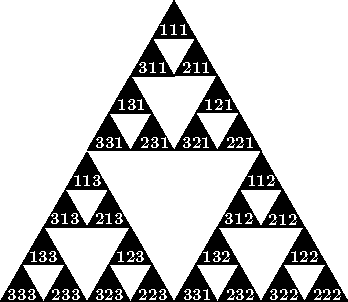
\includegraphics[width=\textwidth]{../img/sierpinski-codes.pdf}
    \caption{}
    \label{fig:sierpinski-codes}
  \end{subfigure}  
  \hspace{0.015\textwidth}
  \begin{subfigure}[b]{0.48\textwidth}
    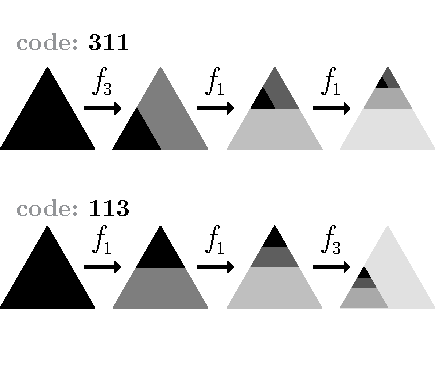
\includegraphics[width=\textwidth]{../img/code-construction.pdf}
    \caption{}
    \label{fig:code-construction}
  \end{subfigure}

  \caption{\small (a) Codes of length three on the Sierpinski triangle and the subsets they code for. (b) The construction of a subset from its code.}
  \label{fig:codes}
\end{figure}

Let $(\sigma_i)$ be a sequence with $\sigma_i \in [1, n]$ for some IFS $S$ with $n$ components. We can compose the components of the IFS acording to the elements of $\sigma$. Call this function $S_\sigma$:
\[
S_\sigma = S_{\sigma_1} \circ S_{\sigma_2} \circ \ldots \circ S_{\sigma_m}
\]

Since each $S_i$ is contractive, we can let the length of $\sigma$ go to infinity and get 
\[
S_\sigma(X) = x_\sigma  
\] 
That is, the sequence of functions maps any non-empty $X$ to a unique point $x_\sigma$. In the case of probability measures, every probability measure is mapped to a probability measure that gives the single point $x_\sigma$ full probability mass. Figure \ref{fig:codes} illustrates the concept: an Iterated Function System assigns a code to each point on its support. Finite codes map to subsets of the support. Since the size of the subsets decreases exponentially we can talk about the endpoint of a finite code without losing much accuracy. We will take the point to which the origin is mapped by $S_\sigma$ as the canonical choice of the endpoint of finite $\sigma$.

Finding the endpoint for given code is straightforward, but we will also require the inverse process: given a point $x$ on or near the support of some IFS, we wish to find $\sigma$. To this end we start with the standard  multivariate normal distribution and apply all maps $S_\sigma$ for all $\sigma$ of a given length $l$ giving us a set of $k^l$ normal distributions (since an affine transformation of a normal distribution is also a normal distribution). The $\sigma$ which assigns $x$ the greatest probability density is chosen.

Since the variance of the distribution drops off exponentially as the length $l$ is increased, this method will fail if points are too far off the support of the IFS (even if logarithmic probabilities are used). To increase the range of the method, we fall back on the distance from the point to the mean of the distribution. If the first method cannot distinguish between codes, we choose the code whose probability distribution has its mean closest to $x$ (this is equivalent to the approximation method described in section \ref{sec:density}).

A word of caution on codes is appropriate: the ordering is often the reverse of what our intuition suggests. If we number the three components of the Sierpinski triangle clockwise from the top 0, 1 and 2, we might number a small section of the triangle by first moving into the top subtriangle, then into the left subtriangle (2) of that and then into the right subtriangle (1) of that. Intuitively, this is the most natural way of coding sections of the Sierpinski triangle.

If we wish to map the whole triangle to this subset, we must reverse the codes: the transformation that maps to the smallest subsection must be applied first. The sequence of transformations which will map the whole triangle into the required subspace is:
\[
S_1(S_2(S_0(x)))
\]
so its code $\sigma$ is $(1, 2, 0)$. If we wish to `travel into' the Sierpinski gasket by this code, we must read it right-to-left.

Finally, we wish to note that a line segment, the square, the cube and higher dimensional analogues can be represented as simple IFSs of $2^d$ components. For instance, for the unit line, we map the whole onto its lower and upper half with two components. The codes of this IFS are binary strings and the subsets they code are the diadic intervals. For the square, we can map the whole onto each one of its quadrants and get quaternary codes. Using this mechanism we can always map any dataset into the bi-unit hypercube and find a straightforward coding for the instances in $2^d$-ary codes. What fractal fitting offers us is a potential for a subspace that fits the data more compactly (ie. using fewer components) and gives us a good code of lower arity.

\subsection*{Calculating density}
\label{sec:density}

The probability density of a given point $x$ under a given IFS model $S$ is straighforward to calculate. For a given depth, we start with a basis MVN $N(x)$ , and calculate the following sum:
\[
\sum_{\sigma \in \{1, \ldots, k\}^l} w_\sigma S(N)(x)
\]

That is, we transform the basis function by $S_\sigma$, the composition of the components of $S$ in the order indicated by $\sigma$ (the endpoint distribution), we weight this value by the $w_\sigma = \prod_{i \in \sigma} w_i$ (the endpoint prior) and sum over all possible $\sigma$.

Clearly, this succession will quickly foce each endpoint distribution to a single point, and only points near one of the models' end points will have a probability that is distinguishable from zero in standard 64-bit floating point representation.

To deal with this situation, we also use an approximated density, which can be used when the correct density approximation yields zero. Of course, we must be careful only ever to compare two correct densities, or two approximated densities, but never to mix the two.

For the approximated density, we only visit the end points $S_\sigma(\mathbf{0})$ of the IFS model, forgetting the endpoint distributions. We place an MVN at this endpoint with a variance of $\rho^l$. We then sum the densities under these distributions, weighted by the endpoint priors $w_\sigma$. So that the approxiamted density becomes:

\[
\sum_{\sigma \in \{1,\ldots,k\}^l} w_\sigma N(x | S_\sigma(\mathbf{0}), I\rho^l)
\]

For our experiments we use $\rho = 0.9$.

% The standard way of evaluating the fit of a model to a dataset is the likelihood of the model given the data. This is often used in optimization algorithms for fitting probability models to data. In the case of fractal models, the likelihood function has an important drawback. 

% Consider a dataset drawn from the Sierpinski gasket with a minute amount of two dimensional noise added. Since the Sierpinski gasket has dimension less than two, the probability that the point will still fall within the Sierpinski gasket will be zero. Thus all points will have probability zero under the Sierpinski gasket and its likelihood will be zero. Intuitively however, the Sierpinski gasket is still a good model for this data.

% For this reason we will often use the Hausdorff distance to evaluate our models. The Hausdorff distance  $H(X, Y)$ between two sets $X$ and $Y$ is defined as follows:
%\[ 
%H'(X, Y) = \max_{x\in X} \, \min_{y\in Y} \, d(x, y) 
%\]
%\[
%H(X, Y) = \max\left (H'(X, Y), H'(Y, X)\right )
%\]
% where $d(\cdot, \cdot)$ is the Euclidean distance. For infinite sets the $\max$ and $\min$ functions should be replaced with $\sup$ and $\inf$.
 
% The most intuitive way of understanding the Hausdorff distance is as a game where the first player must get from one set to the other in as small a distance as possible, and the malevolant second player will choose his starting point to maximize that distance.

% Hausdorff distance is a common tool in dealing with the fractal inverse problem \cite{nettleton1994evolutionary}. We will use it to evaluate an IFS model by generating a number of points from the model and calculating the Hausdorff distance of that set to the model. Since the Hausdorff distance has not been substantiated as a statistical measure, we can only use it as an intermediate indication of model quality. To prove the utility of IFS models we will test them on classification and dimensionality reduction tasks.

\subsection*{Dimension}

The \textit{curse of dimensionality} is a blanket term for many effects related the analysis of high dimensional data. The main cause of these problems is that as dimensionality increases, the volume of a subspace (such as the unit ball) increases exponentially with it. This means, for instance, that vast amounts of samples are required to maintain the same level of coverage in a high dimensional space as compared to a low dimensional one. 

The solution to many of these problems is that while the data has a high-dimensional representation, it has a low intrinsic dimension ('The blessing of self-similarity'). That is, it can be mapped to a low dimensional space without any loss of information. A simple example is that of all points lying on a line in some high dimensional space. 

IFSs have a particular advantage over classical models like Gaussian mixtures: their intrinsic dimension varies over the whole range of positive reals. A search through the space of IFSs can return models of any dimension.

We measure the dimension of datasets and data generated from models using Takens' estimator \cite{takens1985numerical}:
\[
D(d_{\mbox{max}}) = -\frac{|A|}{\sum_{a \in A} \ln a} 
\]
Where $A$ is the set of distances between pairs of data points lower than parameter $d_{\mbox{max}}$. We choose $d_{\mbox{max}}$ as the value that produces the lowest Kolmogorov-Smirnov statistic with the probability distribution underlying the Takens estimator. This method is based on the work for general power laws in \cite{clauset2009power} and will be detailed in a later publication. 

We estimate the uncertainty of this estimate as follows: bootstrap a version of the dataset by sampling to the same size with replacement, and estimate the dimension of that dataset. We repeat the process 50 times and take the sample standard deviation as an estimate of the uncertainty.

\subsection*{Analogous model: Mixture of Gaussians}

To study the IFS as a statistical model, it helps to have a commonly used analogous model to compare it with. We use the Mixture of Gaussians (MoG) model. This model consists of $n$ multivariate Gaussians over ${\mathbb R}^d$ each represented by a mean $\mu \in {\mathbb R}^d$ and a $d \times d$ covariance matrix $\Sigma$. Each component also has a prior $w_i$. The complete model describes the following probability distribution:
\[
p(x) = \sum_{i \in [1,n]} w_i N(x|\mu_i, \Sigma)
\]
Since every multivariate Gaussian can also be described as an affine transformation of the standard normal distribution (mean at the origin and $\Sigma$ the identity matrix), we can also represent the mixture of Gaussians as $n$ affine transformations and $n$ weights, just as the IFS:
\[
p(x) = \sum_{i \in [1,n]} w_i S_i(N(0, I))(x)
\]
This gives us a classical model with a similar representation. Note that the representation would be equal if we used similarities for the MoG model. However since an MVN transformed with uniform scaling is rotationally symmetric that would make all the rotational parameters useless. For this reason we will allow the MoG model full affine transformations as parameters and the IFS model only similarities. Even with this discrepancy, we still consider the MoG to be a reasonable analog.

Unlike the single MVN distribution, there is no closed form solution for the maximum likelihood fit of a MoG model to data. We must approximate it. The most common method is by the well-known EM algorithm. Since our solution to the fractal inverse problem takes inspiration from this algorithm, we describe it here briefly. The key intuition behind the EM algorithm is that if we knew which component of the MoG model `generated' each datapoint, we would have a closed form solution for the parameters of the component, and if we knew the parameters of the components we could find out which component was most likely to have generated the data point. We turn this circular dependency into an iterative algorithm. Starting with some initial MoG model we iterate the following steps

\begin{description}
  \item[Expectation] Assign each data point a probability distribution over the components of the MoG model proportional to the likelihood of the model given the datapoint. In other words, each component takes a certain amount of `responsibility' for the data point.
  \item[Maximization] Estimate the parameters for each component based on the probability weights calculated in the previous step.
\end{description} 

\section*{Fitting IFS models to data}

We can now describe the central algorithm of this paper. To make the explanation as clear as possible we will first describe a skeletal version of the algorithm that works in principle and then describe various alterations to this skeleton that are required to improve the performance of the algorithm on real data with finite approximations of the IFS measures. 

The results described are always for the full algorithm with all improvements. An implementation of only the basic algorithm should be enough to retrieve the Sierpinski gasket (or a crude approximation) from data.

\subsection*{The basic algorithm}

As with the EM algorithm for MoG models, the main barrier to inducing an IFS model from the data directly is a dependency on latent variables. In the MoG case each data point needed to be assigned to a component, in the IFS case we need to know, for each data point the code $\sigma$ that represents the sequence of components. 

Given these codes it's a relatively simple matter to find which points maps to which under the data's self-similarity. And given two ordered lists of points that are supposed to map into one another we can easily find a map to minimize the error. Thus our algorithm works as follows. 
\footnote{the names `expectation' and `maximization' of these steps are only by analogy with the EM algorithm for MoG models. We do not claim any true expectation or maximization procedures.}

\begin{itemize}
\item We start with an initial IFS $S$, chosen by one of the methods described below. 
\item (Expectation) We assign each datapoint a code $\sigma$ of length $d$ (where $d$ is a parameter of the algorithm). The codes are provided by the model $S$ as described above. 
\item (Maximization) We know that if a point $x_\sigma$ is mapped using one of our components we have $S_i(x_\sigma) = x_{i\sigma}$. That is, the symbol for the mapping component is prepended to the code. For each $x_\sigma$ in our dataset we search the data for a point with a code $\tau = i\sigma_{1:k-1}$, the symbol $i$ followed by the elements of $\sigma$ save for the last. For each $i$ we maintain ordered lists of the matches found.
\item (Maximization) For each component $S_i$ we now have two lists of points such that $S_i$ should map one into the other with minimal squared error. We used the method described in \cite{umeyama1991least} to find $S_i$. 
\end{itemize}

We will often use a subsample of the data, for performance reasons. In such cases, we resample for each EM iteration.
 
\subsection*{Improvements}

\subsubsection*{Centering and scaling the data}

Iterated function systems are not very good at approximating data that is weighted far from the origin. For this reason we find the affine transformation which maps the data to the range $[0,1]$ in each dimension.

We store this transformation with the model to map the model back to the data space as needed.

\subsubsection*{Using all depths}

The algorithm as described here can work at all depths $d$. Since each depth may contain information about self similar scaling in the data, we also want to consider all depths less than $d$ rather than just $d$. This is easily done by considering codes of all length up to and including $k$. We build a code tree of the codes generated from the dataset and search it systematically for the required matches at all levels.

% This means that for each $i$ we have two sets of points at each depth. If the components are equally weighted, we will have a set of about $1/n$ of the data, mapping into a set of about $1/{n^2}$ of the data. At depth two the ratios become $1/{n^2}$ and $1/{n^3}$ and so on. For large depths, only specific codes will have matching points.


\subsubsection*{Weights}

The algorithm as described above does not give us a way to retrieve the component weights. For the coding step we already take the weights into account, so the only thing we must do is retrieve them from the set of codes with which we start the maximization step.

If we have a collection of points $X_\sigma$ with code $\sigma$ and a collection of points $X_\tau$ with code $\tau$ such that $S_i$ should satisfy $S_i(x_\sigma) = x_\tau$, we know that if we generate the IFS model, $w_i$ of the probability mass at stage $t$ always gets distributed to component $S_i$ for stage $t + 1$. Thus we can expect the relative size of these sets to follow $w_i$: $|X_\tau| = w_i |X_\sigma|$. Over all such sets $X_\sigma^j$ and $X_\tau^j$ we must minimize the squared error:
\[
\overline{w_i} = \argmin_{w_i} \sum_{j} \left( |X_\tau^j| - w_i |X_\sigma^j| \right)^2
\]
This works out as 
\[
\overline{w_i} = \frac{\sum_{j}|X_\sigma^j||X_\tau^j|}{\sum_{j}|X_\sigma^j|^2}
\]

\subsubsection*{Multiple matches ($\sigma$)}

It is perfectly possible that we get multiple data points which are assigned the same code. Indeed, at low depths, it is almost certain. In this case we have two sets of points $X_\sigma$ and $X_\tau$ such that the points in the former should map onto the latter. But our algorithm for finding the map $S_i$ requires the individual points to be matched to each other. If the number of points is low we can simply take the mean of both sets, but if the number of points is high, we risk throwing away a lot of information (in particular about rotation). Theoretically each point in the first set should map onto every point in the other but this creates an explosion of possiblities. If we pair the points up randomly we introduce artifacts in the induced rotation.

We tackle this problem by finding the MVN for both sets. Ideally we would then extend our method for finding maps to paired MVNs rather than paired points, but this is a highly complex problem. Instead, we make use of the correspondence between MVNs and affine maps. We find for each MVN the transformation that transforms the standard distribution ($N(0, I)$) into that MVN. We then generate $|X_\tau|$ `spanning points' from some initial distribution and map these to both sets. We add these point pairs to the list of matched points from which the maps will be calculated.

To generate the spanning points we use a spherical MVN with variance $\sigma$. This value becomes an important parameter in the algorithm. If the spanning points have a high variance, then the rotation becomes a more important part of the found affine map. The limiting case with $\sigma \rightarrow 0$ is essentially equal to just using the mean of all points with a given code and getting no rotation information from the mapping between single code pairs.

The behaviour of the algorithm under varying $\sigma$ is somewhat mysterious, but trial-and-error testing suggests that for high values the algorithm is more likely to converge. This comes at the cost of some solutions, as with $\sigma = 1.0$, the algorithm is unable to find the two-component Koch curve. For all experiments reported in this paper we use $\sigma = 0.1$. [@! No we don't]

\subsubsection*{Edge cases}

As with standard EM algorithms, some undesired behavior can emerge when the initial model is far from the optimum. Consider for instance the case where the Sierpinski triangle is the current model and all data is to the top right of the triangle. The symbol 2 would not occur in any of the codes and we would have no basis to find $S_2$ in the maximization step. If this occurs, we will `split' one of the components that could be found  (distributing the weight equally) and perturb each component slightly to ensure that the components differ. The idea behind this approach is simple. For every place in every code that used to be assigned to the original component there is now around a fifty/fifty probability of the place being assigned to the other code. In the next step roughly half of the matches of the component will have been `donated' to the other component.

The perturbation is done by flattening the model into a vector of values in ${\mathbb R}$ and adding a small random value $N(0, \pi)$ to each. In our experiments $\pi$ was set to 0.3. 

\subsubsection*{Use the data as a basis}

When we generate a sample from the model (to a fixed depth, rather than with the chaos game), and when we compute the probability density to a fixed point, we make use of some initial normal distribution. As the depth increases the influence of the choice of initial distribution increases exponentially. For low depths, however, our choice can affect the quality of our model. 

To determine our what our initial model should be, we examine the situation for depth one. In this case, our data points get a code of one symbol, and the transformations induced are those that optimally map the whole dataset to these subsets. The equivalent MOG model fits a normal distribution to each subset. For these normal distributions to be the result of a depth one IFS model, we must choose as its initial distribution the MVN fit to the data. With this choice, the MOG model and the MVN model are equivalent (so long as they use the same class of transformations).

To summarize, we choose as our initial distribution an MVN fit for the data restricted to our transformation class. Since we are using Similitudes, we fit a symmetrical MVN to our data, and use that as the initial distribution.

% \subsubsection{Branching}

% [@! Test if this helps]

%As an optimization algorithm, EM is strictly linear in the sense that it only considers a single model at each iteration. To avoid local minima it can often help to evaluate multiple models per iteration. To test whether our algorithm benefits from such additions we introduce a branching mode which works as follows.

%During the iteration of the algorithm we maintain a buffer of models. After each iteration, we generate $b$ versions of the current best model perturbed by a parameter $\sigma$ as with the edge cases. We add these models to the buffer and sort it by Hausdorff distance with the data (as described in section @!). We discard all but the top $h$ models. At the next iteration, we continue with the top model from the list and repeat the procedure.

%This method is analogous with beam search. Its advantage is that we perform the expensive EM step the same number of times as the non-branching model, and the extra cost lies purely in testing evaluating the extra models. (This is not inexpensive in itself, but any branching algorithm will need to test candidate models anyway).

\subsection*{Choosing the initial model}

The choice of initial model is crucial for achieving good performance. The following approaches showed promise in our tests:

\begin{description}
  \item[points] For a model with $k$ components, choose $k$ points from the training data at random. For point $x$, find the transformation which contracts all points to $x$ with a contraction ratio of $0.1$.
  \item[sphere] Choose $k$ random points on the bi-unit sphere in ${\mathbb R}^d$. Continue as with the \textbf{points} method.
  \item[spread] Search (using for instance evolutionary strategies) for $k$ points on the bi-unit sphere so that the sum of their distances is maximized. Continue as before.
  \item[identity] Sample $k$ small perturbations of the identity transformation. Invert if the transformation is not contractive. 
\end{description}

Tests on our datasets show that \textbf{spread} and \textbf{sphere} tend to perform best. Since \textbf{sphere} is the simplest to implement  we use that in all reported results.

\section*{Methods for Random IFS models}

\subsection*{Choice trees}

In the case of fitting deterministic fractals, our main problem turned out to be the existence of a complex hidden variable, in the form of a code for each data point.

In the random case, we are faced with further unobservable information. Assuming that a single dataset is drawn from a given instance of a random fractal ${\cal S}$, we must know how this instance is built up from ${\cal S}$'s deterministic components. To simplify the problem, we will assume that ${\cal S}$'s components all have the same number $k$ of component maps, and that ${\cal S}$ has $m$ components.

The full representation of a single dataset generated from ${\cal S}$ then consists of the generated points (the obeervables), the code tree (with the points at its leaves and a nuber representing the IFS) and at each node of the code tree a number from $\{1, \ldots, m\}$ to denote the choice of component IFS at that level.
 
[@! Picture]

Analogous to the soft responsibilities of the classical EM algorithm, we will use choice trees that hold at their nodes not a single choice of component IFS, but a probability distribution over all components. We'll call these stochastic choice trees.

We now have three elements that together generate a dataset: a discrete RIFS model, codes for each point in each dataset, a choice tree per dataset). Each of these three can be found in a straightforward manner, if the other two are known. Our algorithm consists of an iteration of all three steps.

When we speak of coding, we must now distinguis between the \emph{map coding} of a point, which consists of a string of integers from $(1,k)$ denoting the choice of map of the component IFS at each level and the \emph{complete coding} of a point, which consists of a string of pairs of two integers the frist from $(1, m)$ and the second from $(1,k)$. This code give both the choice IFS component and its map at each level.

[@! algorithm]



\subsection*{Finding codes given a model and a set of choice trees}

\subsection*{Finding a choice tree given a model and a coding}

As we know the coding we can, for each node in the code tree, find the points $X_\sigma$ that have the code prefix $\sigma$. We can also, for every code $\tau$ that extends $\sigma$ by a single symbols, fond the points with that code.

\subsection*{Finding a model given a coding}

Given a complete code for each point, we can repeat the principle used for the 

\section*{Results}

\subsection*{Discrete}
We perform a number of experiments to give an impression of the behavior of IFSs as statistical models, and the EM algorithm as a learning method. 

First, we show a selection of results on 2D datasets to give a visual impression of the behavior of the algorithm. These images represent the value of the EM algorithm over earlier approaches, as methods based on evolutionary algorithms commonly fail to induce fractals from a fractal dataset with this speed or accuracy.

We then investigate the use of IFS models on higher dimensional data. To attempt to visualize the way an iterated function system models a high dimensional dataset, we use a four component model so that we can map the data back to two dimensions and plot it.

\subsection*{Datasets}

\begin{description}
  \item[forest]
  \item[census]
  \item[abalone]
\end{description}

\subsection*{Model fitting and dimension scaling}

\begin{table}[p]
\begin{tabular}{c c c c c}
\hline
data & initial & & & best model \\
\hline
    \includegraphics[width=0.2\textwidth]{../img/runs2d/sierpinski/data.png}
& 
    \includegraphics[width=0.2\textwidth]{../img/runs2d/sierpinski/generation0000.png}
& 
    \includegraphics[width=0.2\textwidth]{../img/runs2d/sierpinski/generation0001.png}
& 
    \includegraphics[width=0.2\textwidth]{../img/runs2d/sierpinski/generation0010.png}
& 
    \includegraphics[width=0.2\textwidth]{../img/runs2d/sierpinski/generation0032.png}
\\
 & & 6 & 48 & 83 \\
    \includegraphics[width=0.2\textwidth]{../img/runs2d/sierpinskioff/data.png}
& 
    \includegraphics[width=0.2\textwidth]{../img/runs2d/sierpinskioff/generation0000.png}
& 
    \includegraphics[width=0.2\textwidth]{../img/runs2d/sierpinskioff/generation0003.png}
& 
    \includegraphics[width=0.2\textwidth]{../img/runs2d/sierpinskioff/generation0020.png}
& 
    \includegraphics[width=0.2\textwidth]{../img/runs2d/sierpinskioff/generation0079.png}
\\    
 &  & 3 & 20 & 79 \\
	\includegraphics[width=0.2\textwidth]{../img/runs2d/koch2/data.png}
& 
    \includegraphics[width=0.2\textwidth]{../img/runs2d/koch2/generation0000.png}
& 
    \includegraphics[width=0.2\textwidth]{../img/runs2d/koch2/generation0008.png}
& 
    \includegraphics[width=0.2\textwidth]{../img/runs2d/koch2/generation0022.png}
& 
    \includegraphics[width=0.2\textwidth]{../img/runs2d/koch2/generation0078.png}
\\    
 &  & 8 & 22 & 78 \\
	\includegraphics[width=0.2\textwidth]{../img/runs2d/ball/data.png}
& 
    \includegraphics[width=0.2\textwidth]{../img/runs2d/ball/generation0000.png}
& 
    \includegraphics[width=0.2\textwidth]{../img/runs2d/ball/generation0003.png}
& 
    \includegraphics[width=0.2\textwidth]{../img/runs2d/ball/generation0024.png}
& 
    \includegraphics[width=0.2\textwidth]{../img/runs2d/ball/generation0072.png}
\\   
 &   & 3  & 24 & 72 \\
	\includegraphics[width=0.2\textwidth]{../img/runs2d/coast/data.png}
& 
    \includegraphics[width=0.2\textwidth]{../img/runs2d/coast/generation0000.png}
& 
    \includegraphics[width=0.2\textwidth]{../img/runs2d/coast/generation0008.png}
& 
    \includegraphics[width=0.2\textwidth]{../img/runs2d/coast/generation0020.png}
& 
    \includegraphics[width=0.2\textwidth]{../img/runs2d/coast/generation0069.png}
\\
 &  & 8 & 20 & 69 \\
\hline 

\end{tabular}
\caption{Selected training steps of the algorithm for various data sets. All models were trained with a dataset of 100000 points, sampling 300 per iteration for 100 iterations. Model depth was 6 for all runs. 1000 points were sampled from each model and from the dataset to estimate the Hausdorff distance (and determine the `best model'). The blue squares indicate the transformations (of the red square) that make up the model. The green bar indicates component weight. By row: (1) The sierpinski triangle, $\sigma = 0.1$ (2) The sierpinski triangle with unequal weights. $\sigma = 0.1$ (3) The 2-component koch curve. $\sigma = 0.001$ (4) A uniform distribution over the bi-unit ball (3 components, $\sigma = 0.1$) (5) Points sampled from a small stretch of coast line (3 components, $sigma = 0.1$). }
\label{tablelabel}
\end{table}


[@! EXPERIMENT for various datasets, for various depths and component sizes, scatter plot the difference between the model dimension and the data dimension against the model accuracy (by hausdorff distance) show uncertainty with error bars]

First, we fit IFS models to our datasets (ignoring the class information). We report the Haussdorff distance of a sample of 1000 points from the data to 1000 points generated by the model (we consider the iris dataset to be too small for this purpose). We withhold a random 25\% of the data for testing, repeat the experiment 20 times and report the sample standard deviation and the mean of the resulting values for symmetric error.

We are also interested in the dimensional scaling of the model. In this case we are interested in the training behavior of the model, so we do not withhold test data. We measure the dimension of the dataset on a random sample of 300 points (repeating 25 times to measure the uncertainty) and generate 300 points from the best model and measure the dimension in the same way. We expect that the difference between the model dimension and the data dimension depends on the quality of the model. Figure @! plots the data dimension against the model dimension. 


In all cases we train the model for 300 generations and select the best model by Hausdorff distance. 

\begin{figure}[t]
\centering

  \begin{subfigure}{0.66\textwidth}
	\includegraphics[width=\textwidth]{../img/dimension/out-table.pdf}
  \end{subfigure}
  \begin{subfigure}{0.33\textwidth}
    \begin{tabular}{c c }
    data & model \\
		\includegraphics[width=0.5\textwidth]{../img/dimension/data-henon.png} & 
		\includegraphics[width=0.5\textwidth]{../img/dimension/model-henon.png} \\
		\includegraphics[width=0.5\textwidth]{../img/dimension/data-ikeda.png} & 
		\includegraphics[width=0.5\textwidth]{../img/dimension/model-henon.png} \\
		\includegraphics[width=0.5\textwidth]{../img/dimension/data-henon.png} & 
		\includegraphics[width=0.5\textwidth]{../img/dimension/model-henon.png} \\
	\end{tabular}
  \end{subfigure}
  \caption{To investigate the dimensional scaling of IFS models, we train them on three generated datasets. The datasets were chosen for a) their low intrinsic dimension, which is easy to measure b) their synthetic nature so that we have an analytic value of their dimension and c) their lack of an accurate IFS approximation, so that the models will not fit perfectly. The datasets are shown on the left with their respective IFS model. They are, from top to bottom: the H\'enon attractor, the Ikeda attractor, and the R\"ossler attractor.}
  \label{fig:dim_scale}
\end{figure}


\subsection*{Classification}

We explore two methods for using IFS models for classification. In the first, we train a single model for each class and combine in a straightforward manner using Bayes' rule. In the second, we learn a single model for the whole set of points, and use the codes generated by the model to perform classification.  

\subsubsection*{Bayesian}

Given some data set $X = \{x_i\} \subseteq {\mathbb R}^d$ with associated classes $c_i \in \{1, 2, \ldots, m\}$, we split the data by class: $X_c = \{ x \in X \mid c_i = c\}$. We train a probability model $p_c$ for each $X_c$ and classify each new point with
\[
C(x) = \argmax_{c} p_c(x) p(c)
\]
The class prior $p(c)$ is estimated as $\frac{|X_c|}{|X|}$.

\subsubsection*{Single model}

An alternative way to construct a classifier with IFS modelling is to learn a single model for the whole dataset, ignoring class labels. For some datasets, the set of all points may present a more coherent and simple distribution than the sets split by class label. Another advantage of this approach is that we only have to learn one model, which is cheaper both in training and in evaluation.

The model provides us with a mapping from the data space (${\mathbb R}^d$) to code space ($\{1, \ldots, k\}^d$). To turn this model into a classifier we proceed as follows. We build a code tree such that each possible code represents a path from the root to the leaf node. We then traverse this tree for each point in the training set, maintaining a frequency count for each class observed at each node. Thus, the root node gives us the frequency distribution over the classes for the whole dataset and each node below it refines that to a distribution over a section of the dataset whose code starts with a given prefix. This turns each node into a very basic classifier, which simply returns the class with the highest frequency count. The root node will give us the classifier that uses nothing more than class frequencies and each node below it will use more information about the neighbourhood of the point.

For each point to be classified we take the probabilities at each node in the path and average them evenly. 

The single model classifier also gives us a good baseline to evaluate how well the model fitting works on natural datasets. As noted before, for any dimension $d$ we can define an IFS model in $2^d$ components which defines a uniform distribution of the $d$-dimensional hypercube. For example, in two dimensions we can start with a square and use the four transformations that map the square onto each of its quadrants. The codes assigned by this model are strongly related to basic spatial indexing techniques, and can be calculated very efficiently. 

The single classifier described above, when used with such codes, classifies based on histograms over a simple binning of the feature space (averaging over various levels of coarseness). It does not perform any dimensionality reduction and very little generalization. We will refer to this method as a spatial index classifier.

If we wish to assert that the EM algorithm for IFS induction results in a meaningful subspace, the single model classifier with an optimized model should perform significantly better than the spatial index classifier. 
 
\begin{table}[h]
\begin{tabular}{| l | r l r l | r l r l  r l r l |}
\hline
  & ifs bayes & & ifs single & & mog & & ann & & knn & & tree & \\
\hline
census  & & & & & & & 0.054 &\color{gray}(0) & 0.06 & \color{gray} (0.002) & 0.05 & \color{gray} (0.001) \\
forest  & & & & & & & 0.163 &\color{gray}(0.001) & 0.138 &\color{gray}(0.001) & 0.12&\color{gray}(0.003) \\
abalone & & & & & & & 0.47 & \color{gray}(0.008) & 0.47 & \color{gray}(0.006) & 0.48 & \color{gray}(0.01) \\
mnist   & & & & & & & 0.09 & & 0.05 & & 0.20 & \\
\hline

\end{tabular}
\caption{Hausdorff distances for models trained against various datasets.}
\label{classification-results}
\end{table}
\subsection{Time performance}

An informal analysis of the algorithm shows that the expectation step costs $O(k^dn)$, with the maximization step taking roughly $O(n^2)$. This falsely suggests that the expectation step, being linear in the number of data points, is negligable compared to the maximization step, which is quadratic. Of course, when viewed in terms of the parameters the expectation step is exponential and this is what causes the expectation step to become the bottleneck for anything but very low values of $k$ and $d$. 

\subsection*{Rnadom}

\section*{Conclusions}

We have presented a framework for a fractal approach to the statistics of point patterns. We introduced an EM-style algorithm for fitting fractal models to data. Compared to search algorithms for other types of models the algorithm is relatively expensive, but compared to other approaches for fractal modeling the algorithm represents a significant improvement [@!]. 

with these tools in place, we believe the door is opened to new opportunities for statistical modeling with fractals. Rather than simply proving that fractal structure exists in a dataset (for instance by measuring its fractal dimension), these algorithms will help researchers to expose that structure. Which datasets and modeling problems are susceptible to fractal analysis of this kind is a question for future research.

\bibliographystyle{siam}
\bibliography{fractal}

\end{document}